\chapter{Theory}

This chapter serves to introduce relevant theory on which the thesis rests. We will briefly review EEG, its use in research and practice. We also briefly review machine learning techniques used on EEG data, in particular Riemannian geometry.

\section{Electroencephalography (\gls{eeg})}\label{eeg-theory}

    % Intro
    Electroencephalography is a method used to measure the activity of neurons in the brain by recording the electrical potential of the scalp. These measurements are performed (sampled) hundreds of times per second, and are then put in sequence to form a signal of what can informally be referred to as ``brain waves''. 

    % Use in medicine & research
    As a non-invasive method it is widely used in medicine to diagnose and study a wide range of conditions, including epilepsy and sleep disorders. 
    It has also found use in research, in particular for studying \glsxtrfullpl{erp}, which are stereotyped responses to a stimulus, an example of which can be seen in Figure~\ref{figure:n170}. Examples of common ERPs can be seen in Table~\ref{table:erps}.

    \begin{table}
        \centering
        \begin{table}
    \centering
    \begin{tabular}{ll}
        \toprule
        ERP & Elicited by
        \\
        \midrule
        N170 & Processing of faces, familiar objects or words.
        \\
        N400 & Words and other meaningful stimuli.
        \\
        P300 & Decision making, oddball paradigm.
        \\
        P600 & Hearing or reading grammatical errors and other syntactic anomalies.
        \\
        \bottomrule
    \end{tabular}
    \caption{Common \emph{Event-Related Potentials} (ERPs)}\label{table:erps}
\end{table}

        \caption{Common \glsxtrfullpl{erp}}\label{table:erps}
    \end{table}

    \begin{figure}
    \centering
    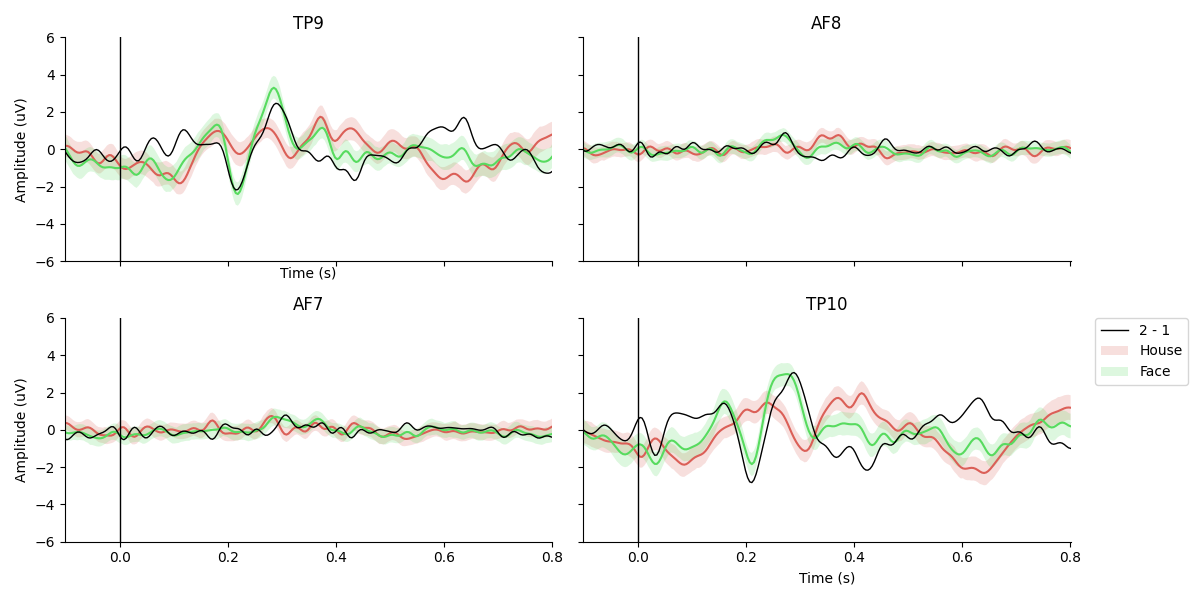
\includegraphics[trim=0 0 80 0, clip, width=14cm]{img/n170_viz.png}
    \caption{Example of aggregated epoch-averaged ERP trials from an N170 experiment, where the subject was shown either a face (in \textcolor{green}{\textbf{green}}) or a house (in \textcolor{red}{\textbf{red}}). The difference between the two stereotyped responses can be seen in black. The vertical line marks the beginning of the epoch.}\label{figure:n170}
    \source{eeg-notebooks \href{https://neurotechx.github.io/eeg-notebooks/auto_examples/visual_n170/01r__n170_viz.html}{experiment gallery} (BSD 3-clause)}
\end{figure}


    One difficulty of working with EEG lies in the low signal-to-noise ratio: measurements are on the order of microvolts, and what is being measured is the electrical activity of some subset of the approximately 86 billion neurons in the human brain. This often leads to signal artifacts from other, non-neural, electrical activity near the scalp, such as that caused by muscle activity from e.g.\ eye blinks (as seen in \Vref{fig:muselsl-signal}).

    The non-invasive nature of EEG can be contrasted with \glsxtrfull{ecog}, a form of \glsxtrfull{ieeg}, which is an invasive method where a craniotomy (a surgical incision on the skull) is performed to implant an electrode grid directly on the cerebral cortex. The result is higher spatial resolution, and improved signal-to-noise ratio due to closer proximity to neural activity. It is almost exclusively used in patients with intractable epilepsy (not responding to anticonvulsants).

    Electrodes can be placed at different locations on the scalp, targeting different regions of the brain. The system used to position the electrodes is called the 10–20 system (seen in Figure~\ref{fig:1020}), and is the standard way to label electrode placements. The \emph{10} and \emph{20} come from the fact that distances between adjacent electrodes are either 10\% or 20\% of the total front–back or right–left distance of the scalp.

    \begin{figure}[h]
        \begin{center}
            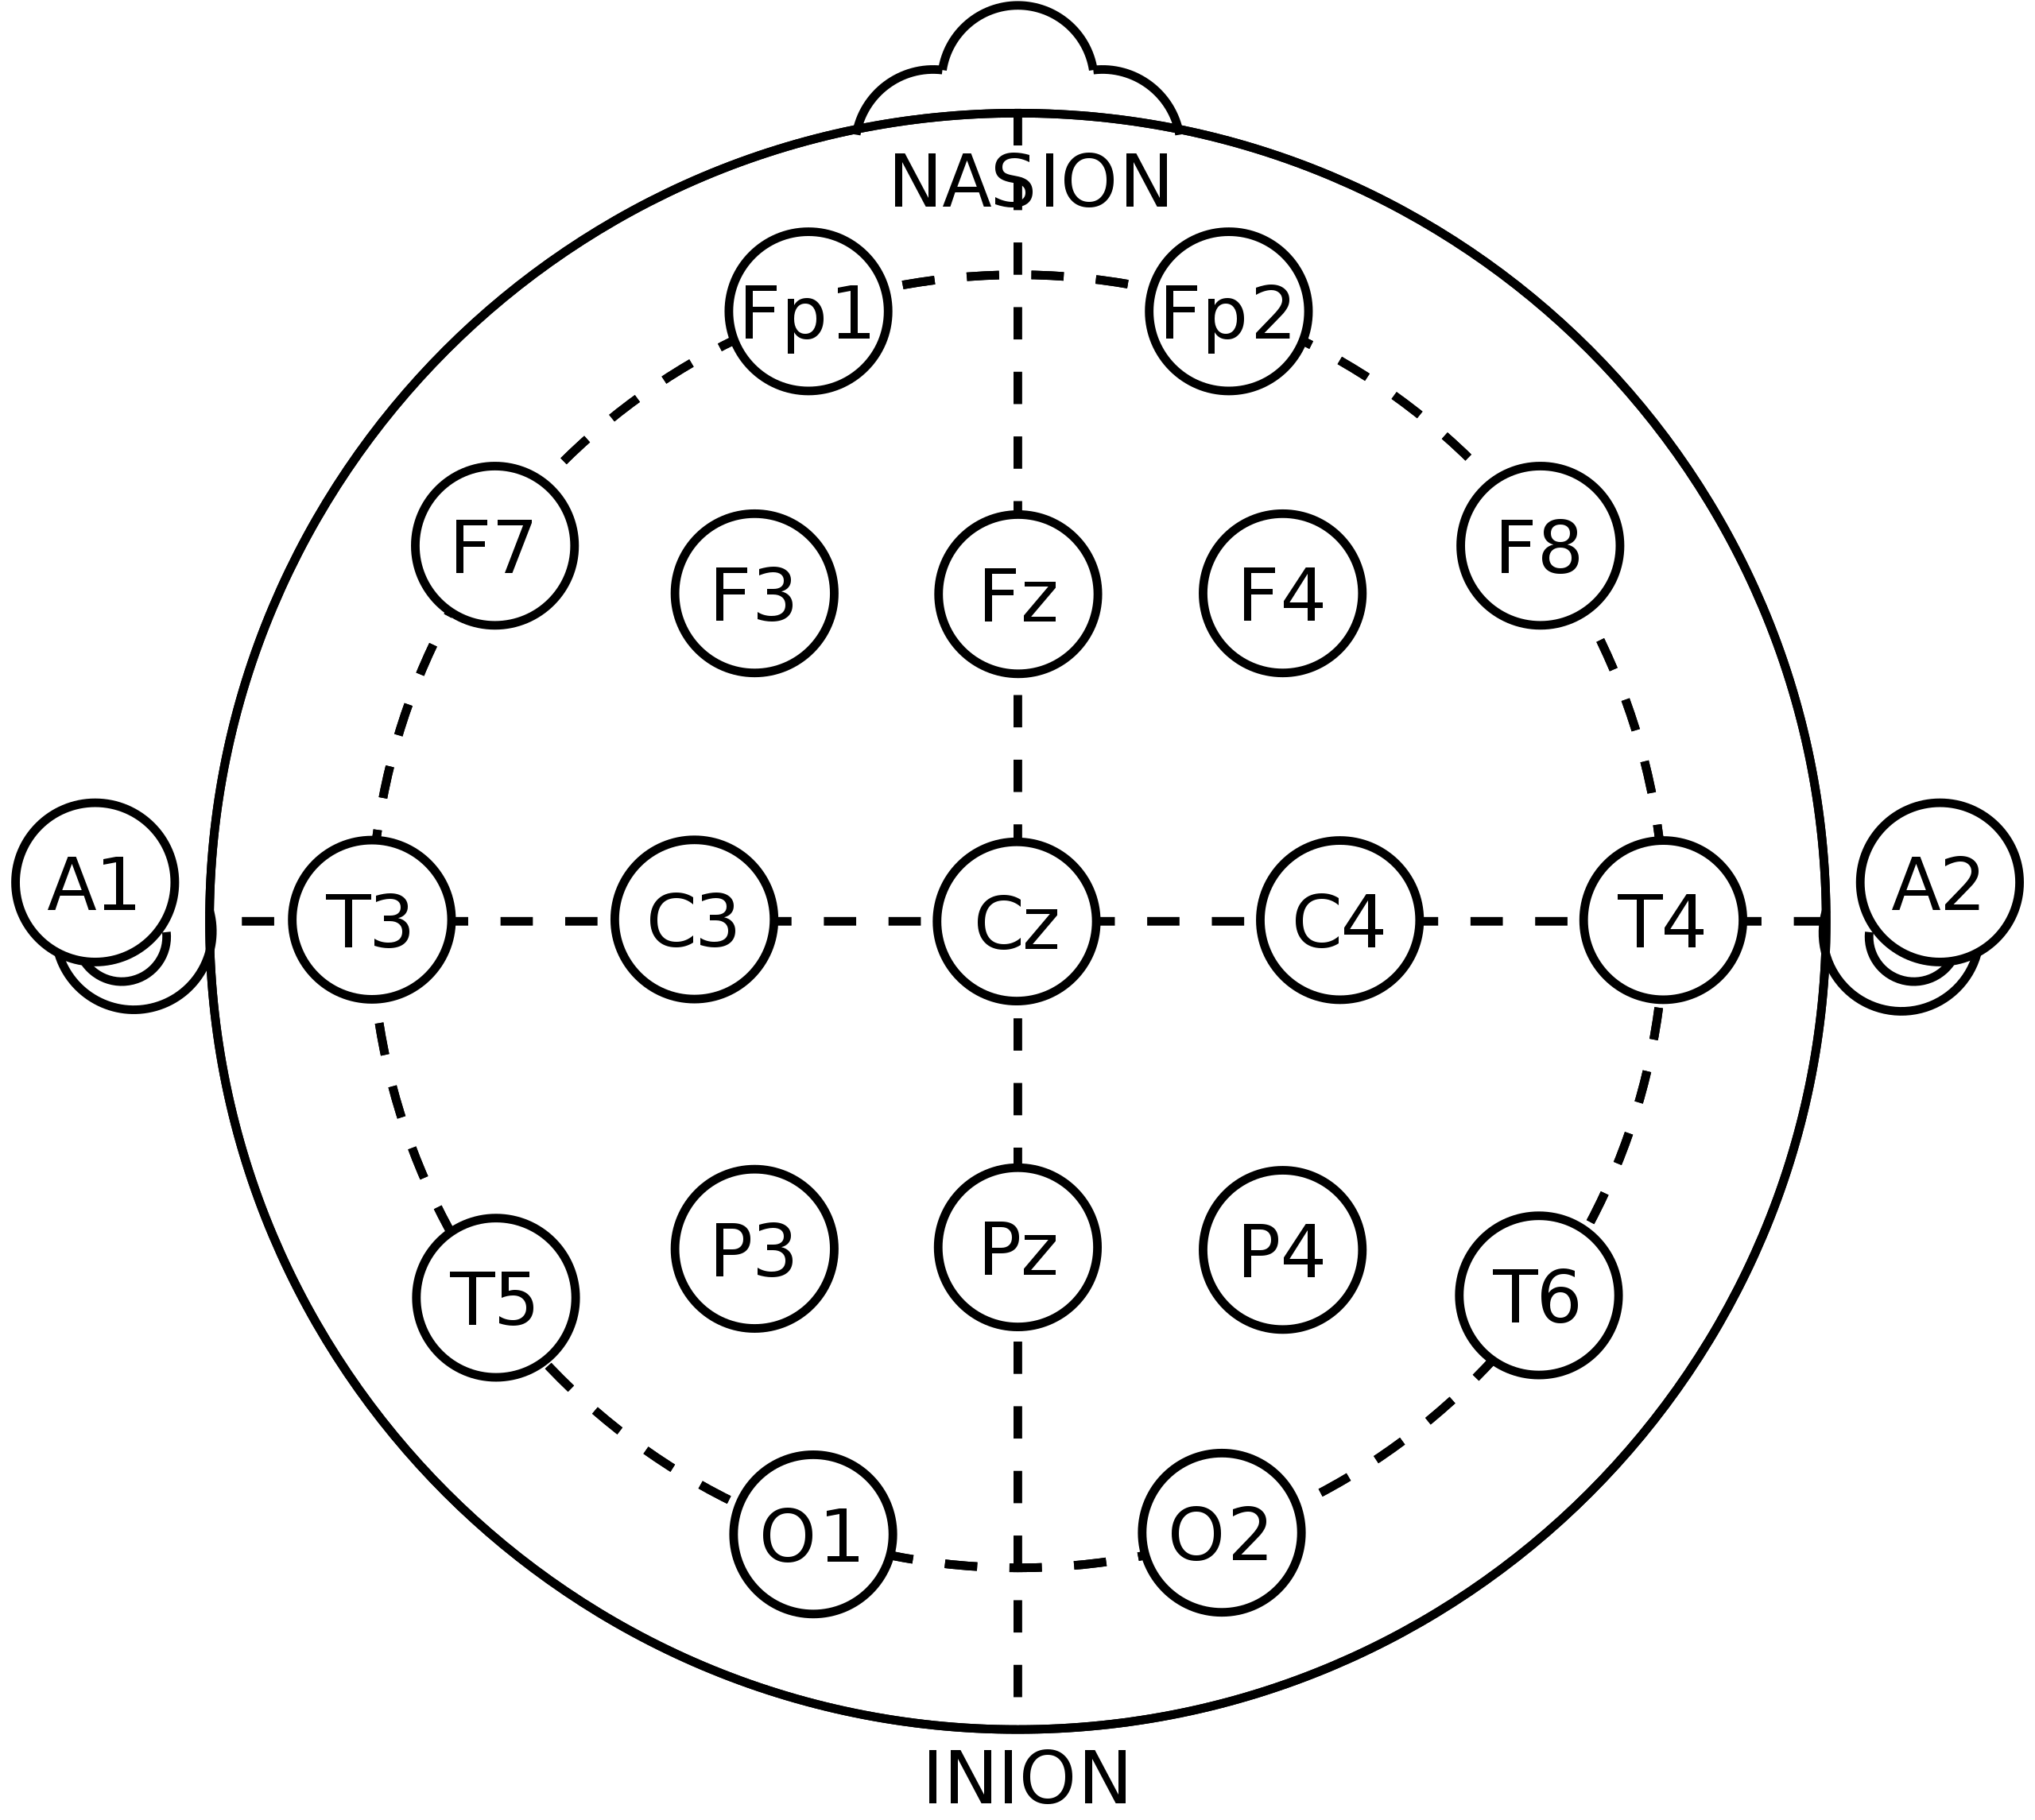
\includegraphics[width=8cm]{img/1020system.png}
        \end{center}
        \caption{The 10–20 system.}\label{fig:1020}
        \source{\href{https://commons.wikimedia.org/wiki/File:21_electrodes_of_International_10-20_system_for_EEG.svg}{Wikimedia Commons} (public domain)}
    \end{figure}

    For configurations with high-density or more specific electrode placement there is also the extended 10--10 system, using \gls{mcn}. In this system, the electrode placements are divided by 10\% increments instead of the usual 20\% (seen in Figure~\ref{fig:1010}).

    \begin{landscape}
        \begin{figure}
            \begin{center}
                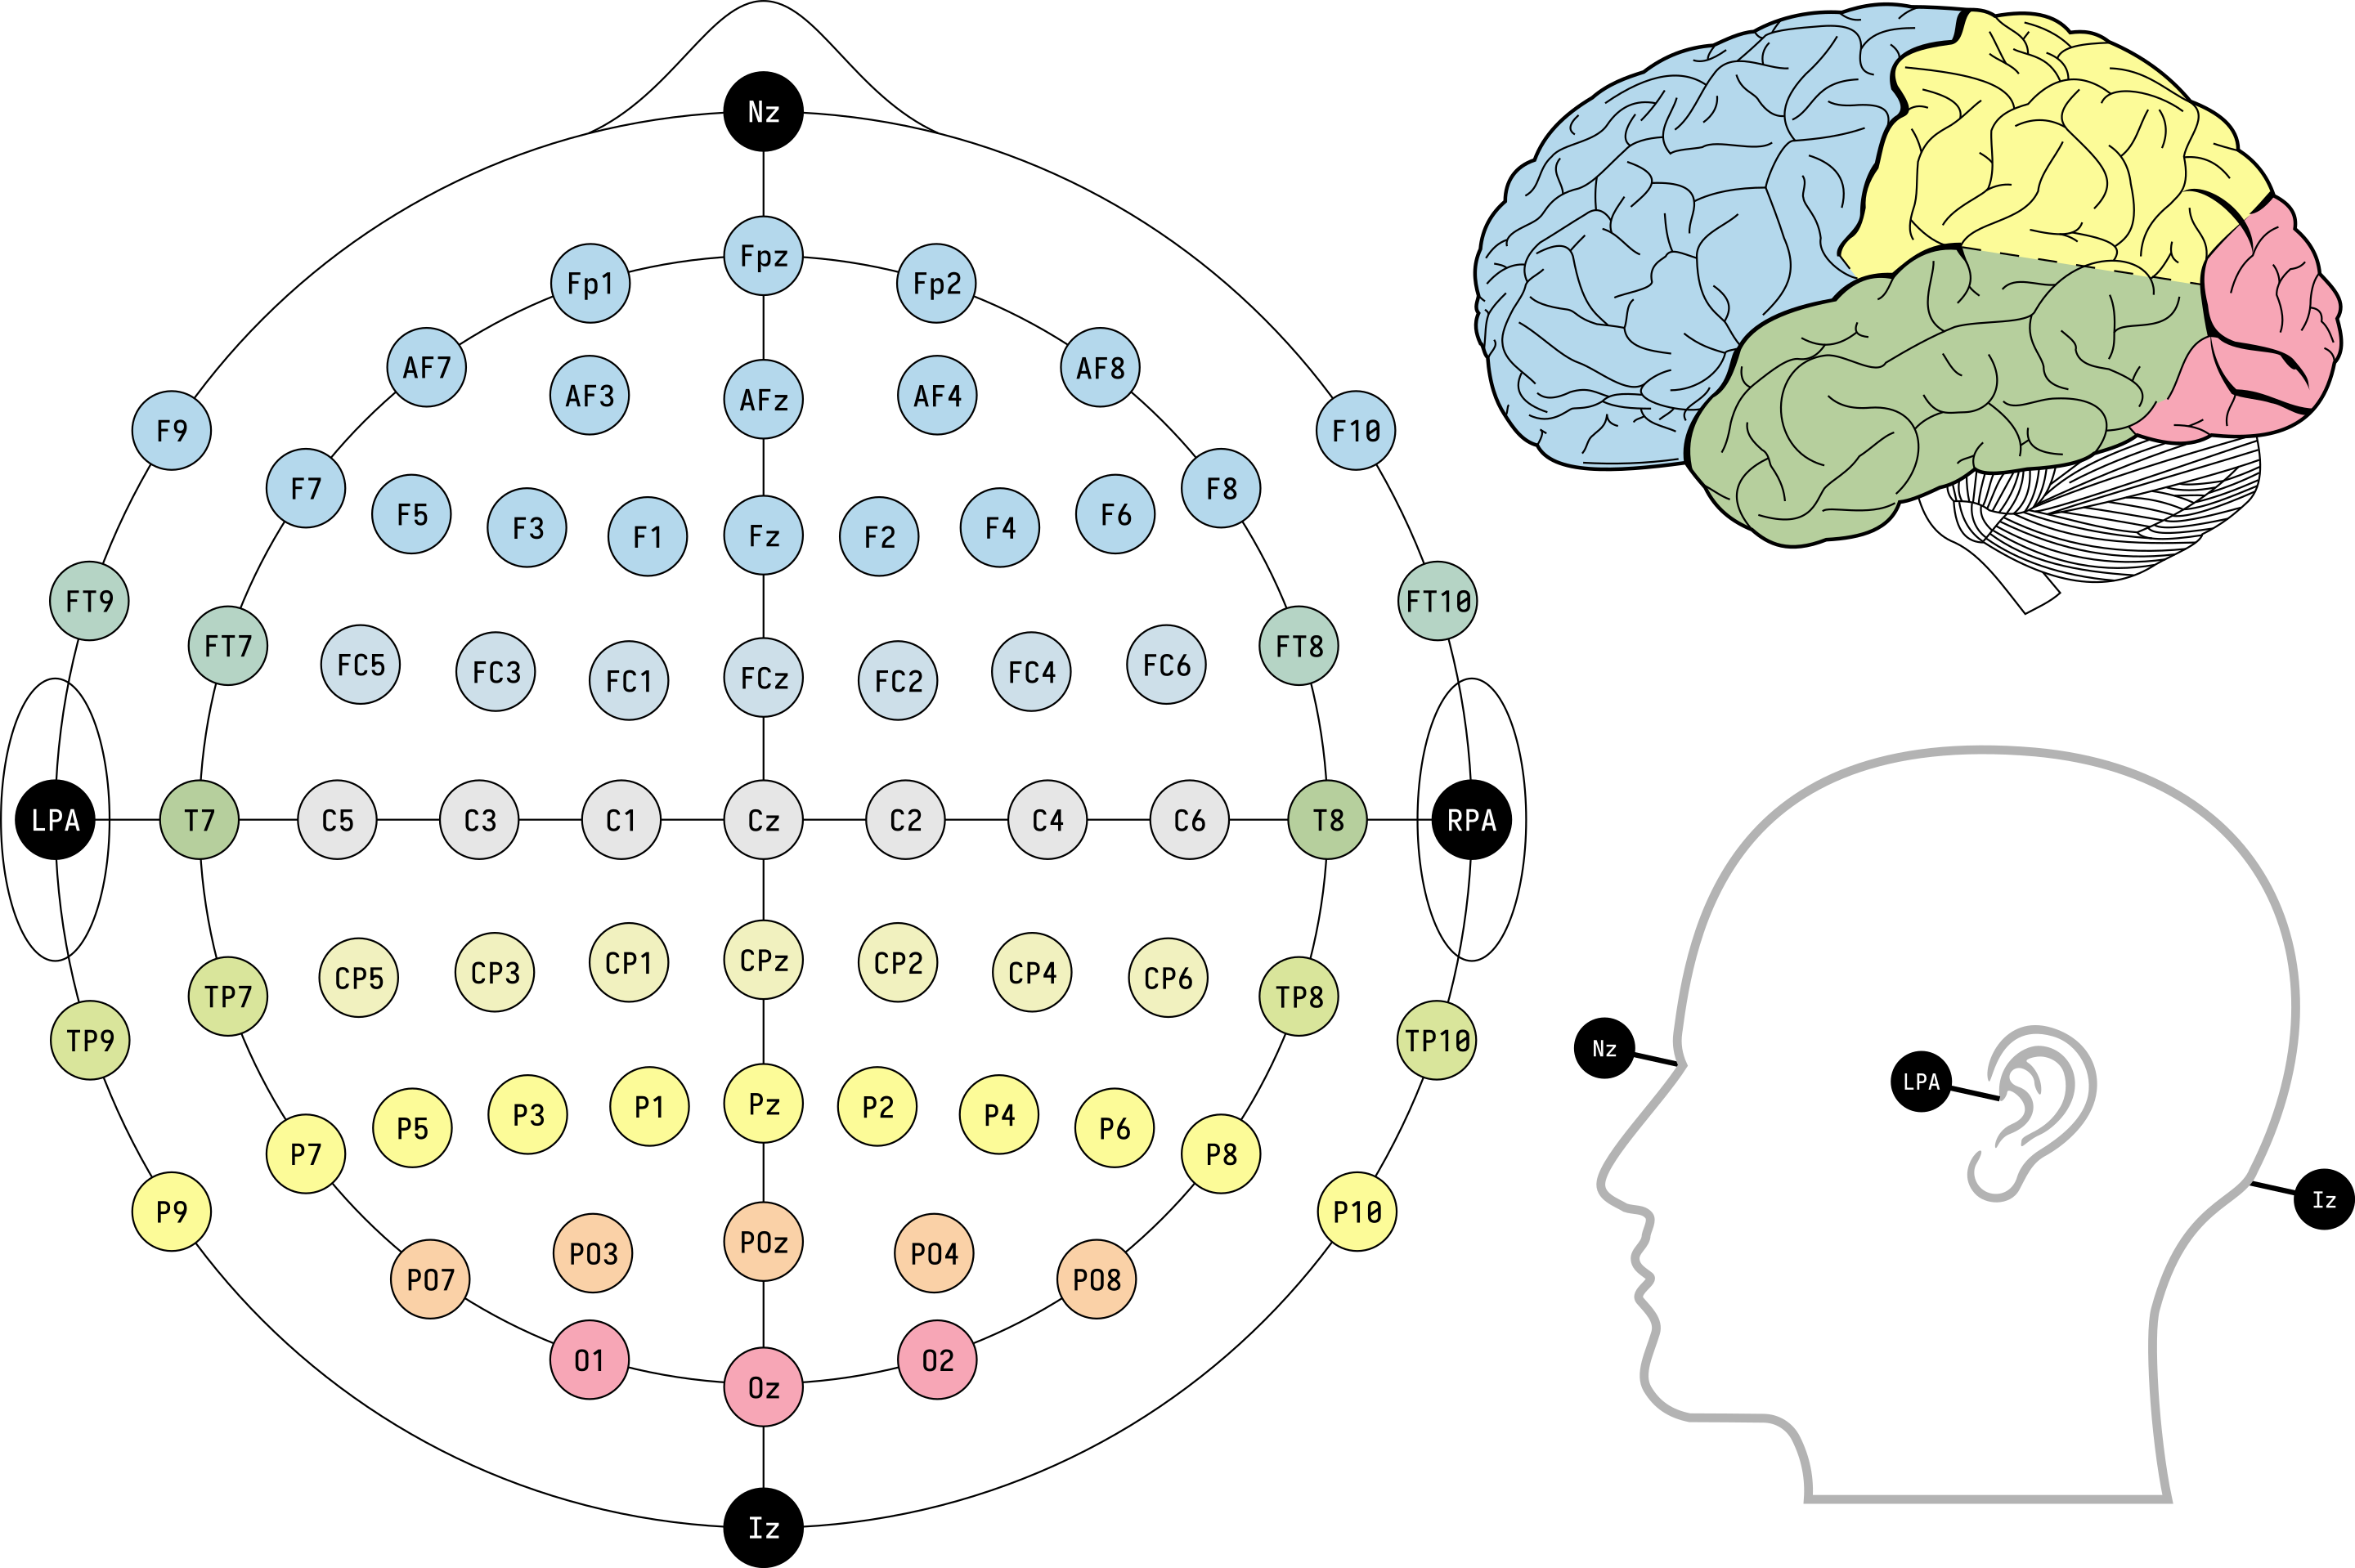
\includegraphics[width=20cm]{img/1020system-extended-with-extra-info.png}
            \end{center}
            \caption{The extended 10–10 system, following the Modified Combinatorial Nomenclature (MCN).}\label{fig:1010}
            \source{\href{https://commons.wikimedia.org/wiki/File:EEG_10-10_system_with_additional_information.svg}{Wikimedia Commons} (CC-0)}
        \end{figure}
    \end{landscape}

    As measurements are taken on the scalp, neural activity of surface-level neurons (such as the cerebral cortex) are expected to dominate the signal, which makes it difficult to use when studying systems deeper in the brain (such as the hippocampus). As an example of this, eye blinks are easily identifiable in the signal when electrodes are placed on the frontal cortex (seen in Figure~\ref{fig:muselsl-signal}).

    %\add[inline]{Plots of PSD, PCA, etc}
    %\add[inline]{Discuss some of the review articles on EEG/BCI/ML}

    Raw EEG data usually contain artifacts from powerline noise, which needs to be filtered out. This is usually done with a simple bandpass filter, an example of which can be seen in Figure~\ref{fig:signal-unfiltered} and~\ref{fig:signal-filtered}.
    
    \begin{figure}[H]
        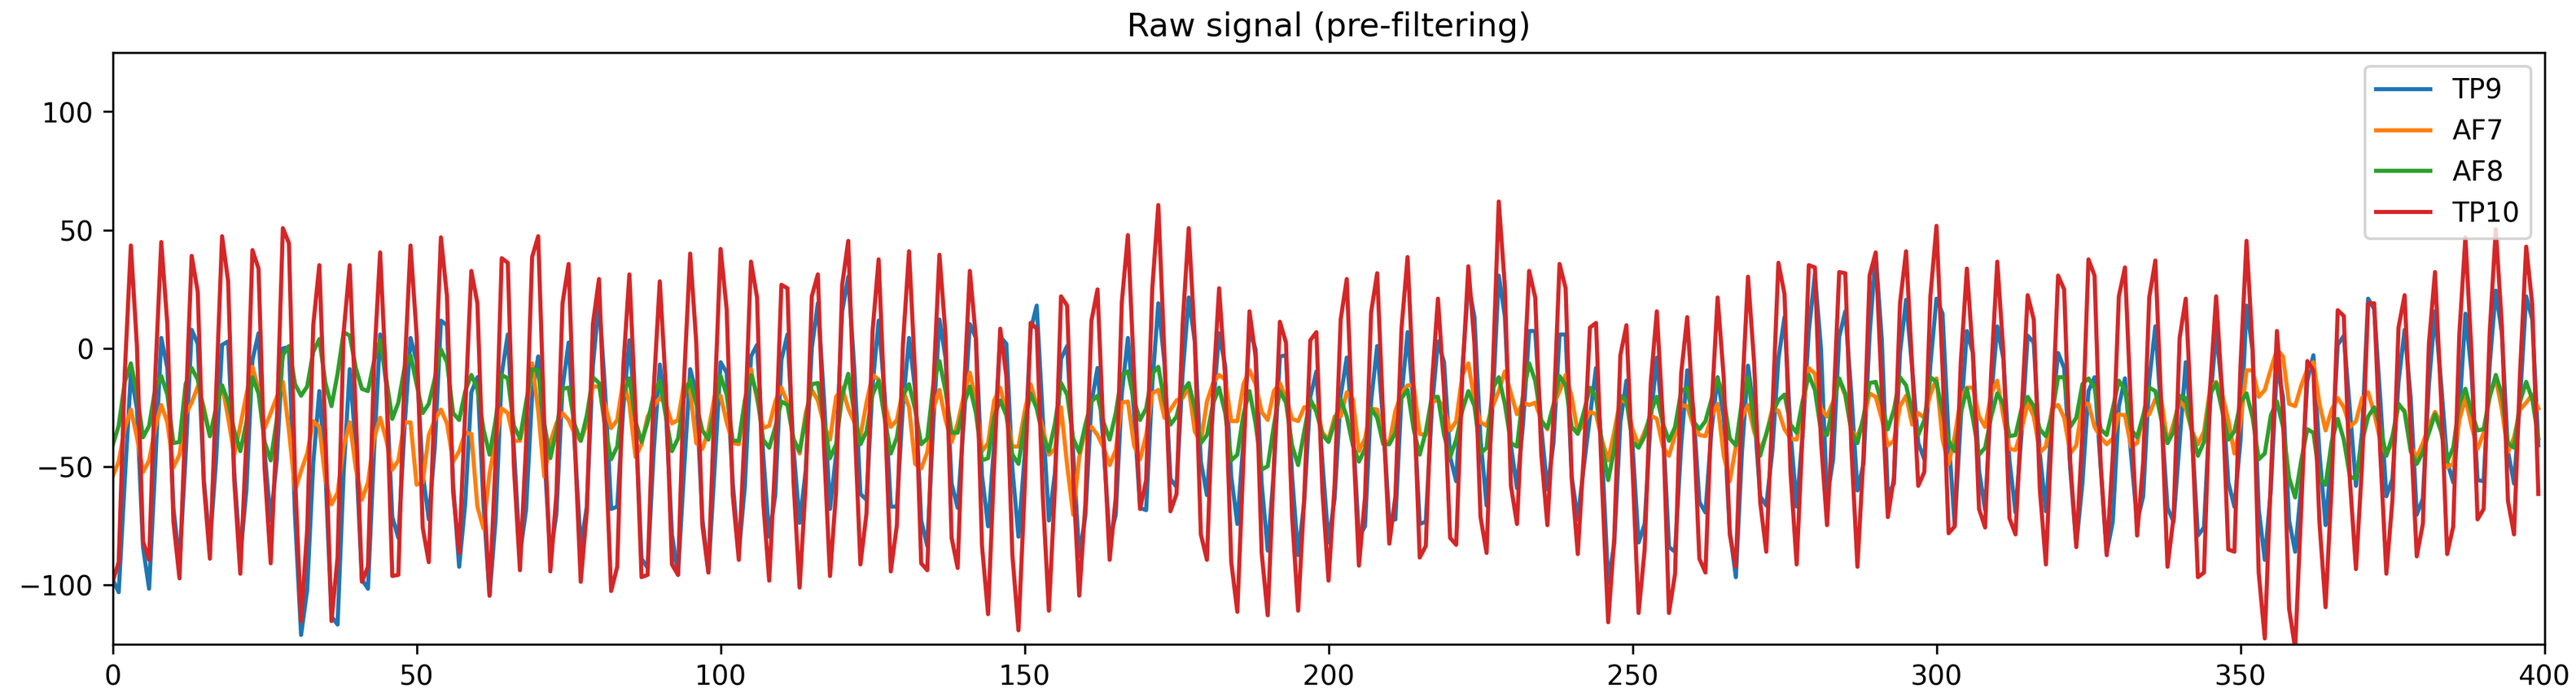
\includegraphics[width=14cm]{img/raw-signal-prefilter.png}
        \caption{Raw EEG signal with no filtering. Powerline noise clearly visible.}\label{fig:signal-unfiltered}
    \end{figure}

    \begin{figure}[H]
        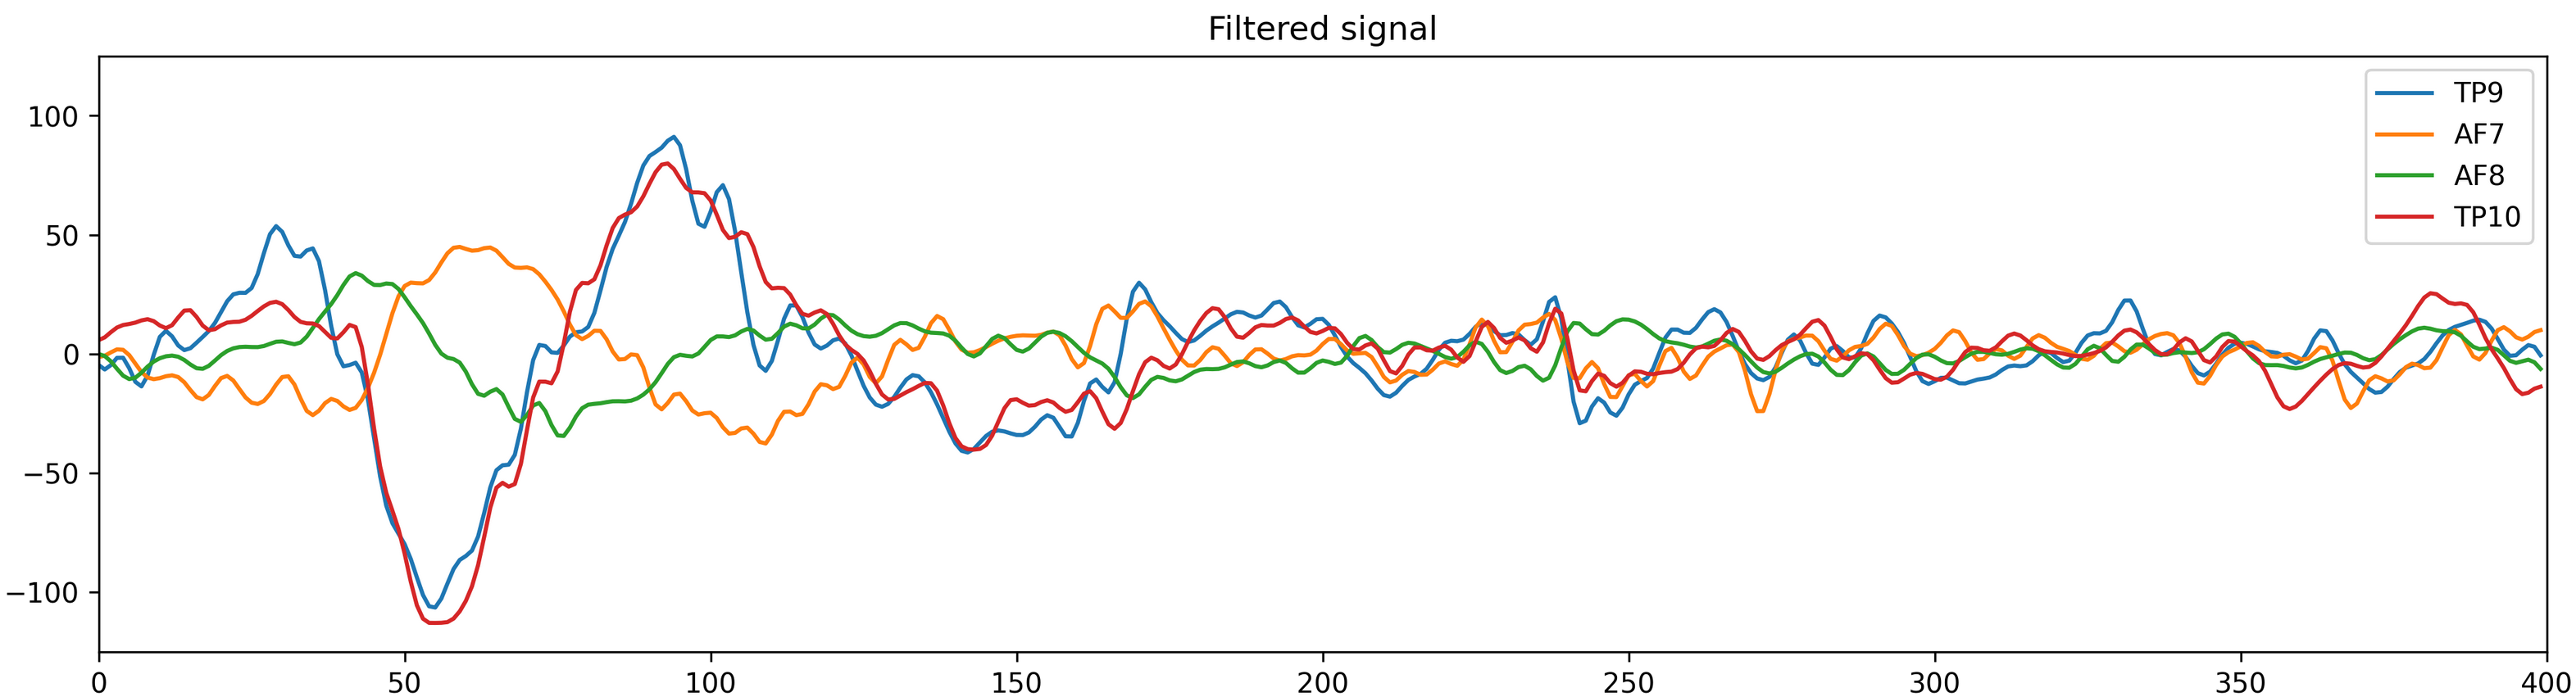
\includegraphics[width=14cm]{img/raw-signal-postfilter.png}
        \caption{Same EEG signal as in Figure~\ref{fig:signal-unfiltered}, but with bandpass filter applied. We can see that powerline noise has been eliminated.}\label{fig:signal-filtered}
    \end{figure}

    After the signal has been filtered, one can perform spectral density approximation to estimate the relative power of different frequency bands in the signal. An example of frequency bands commonly used can be seen in Table~\ref{table:freq-bands}. We will come back to this later in the method, where we use this information as features for one of our classifiers.

    \begin{table}
        \centering
        \begin{tabular}{lll}
    \toprule
    Frequency band & Frequencies & Brain states \\
    \midrule
    Gamma ($\gamma$) & >35 Hz & Concentration \\
    Beta ($\beta$) & 16--35 Hz & Active, external attention, relaxed \\
    Sigma ($\sigma$) & 12--16 Hz & Sleep spindles \\
    Alpha ($\alpha$) & 8--12 Hz & Very relaxed, passive attention \\
    Theta ($\theta$) & 4--8 Hz & Deeply relaxed \\
    Delta ($\delta$) & 0.5--4 Hz & Sleep \\
    \bottomrule
\end{tabular}

        \caption{Characteristics of common frequency bands used in EEG research. Note the \emph{Sigma} band, which is usually grouped with the \emph{Beta} band, but is often used in sleep research where it targets sleep spindles during stage 2 NREM sleep. In some research, these bands are split further into slow and fast counterparts.}\label{table:freq-bands}
    \end{table}

    \begin{landscape}
        \begin{figure}
            \begin{center}
                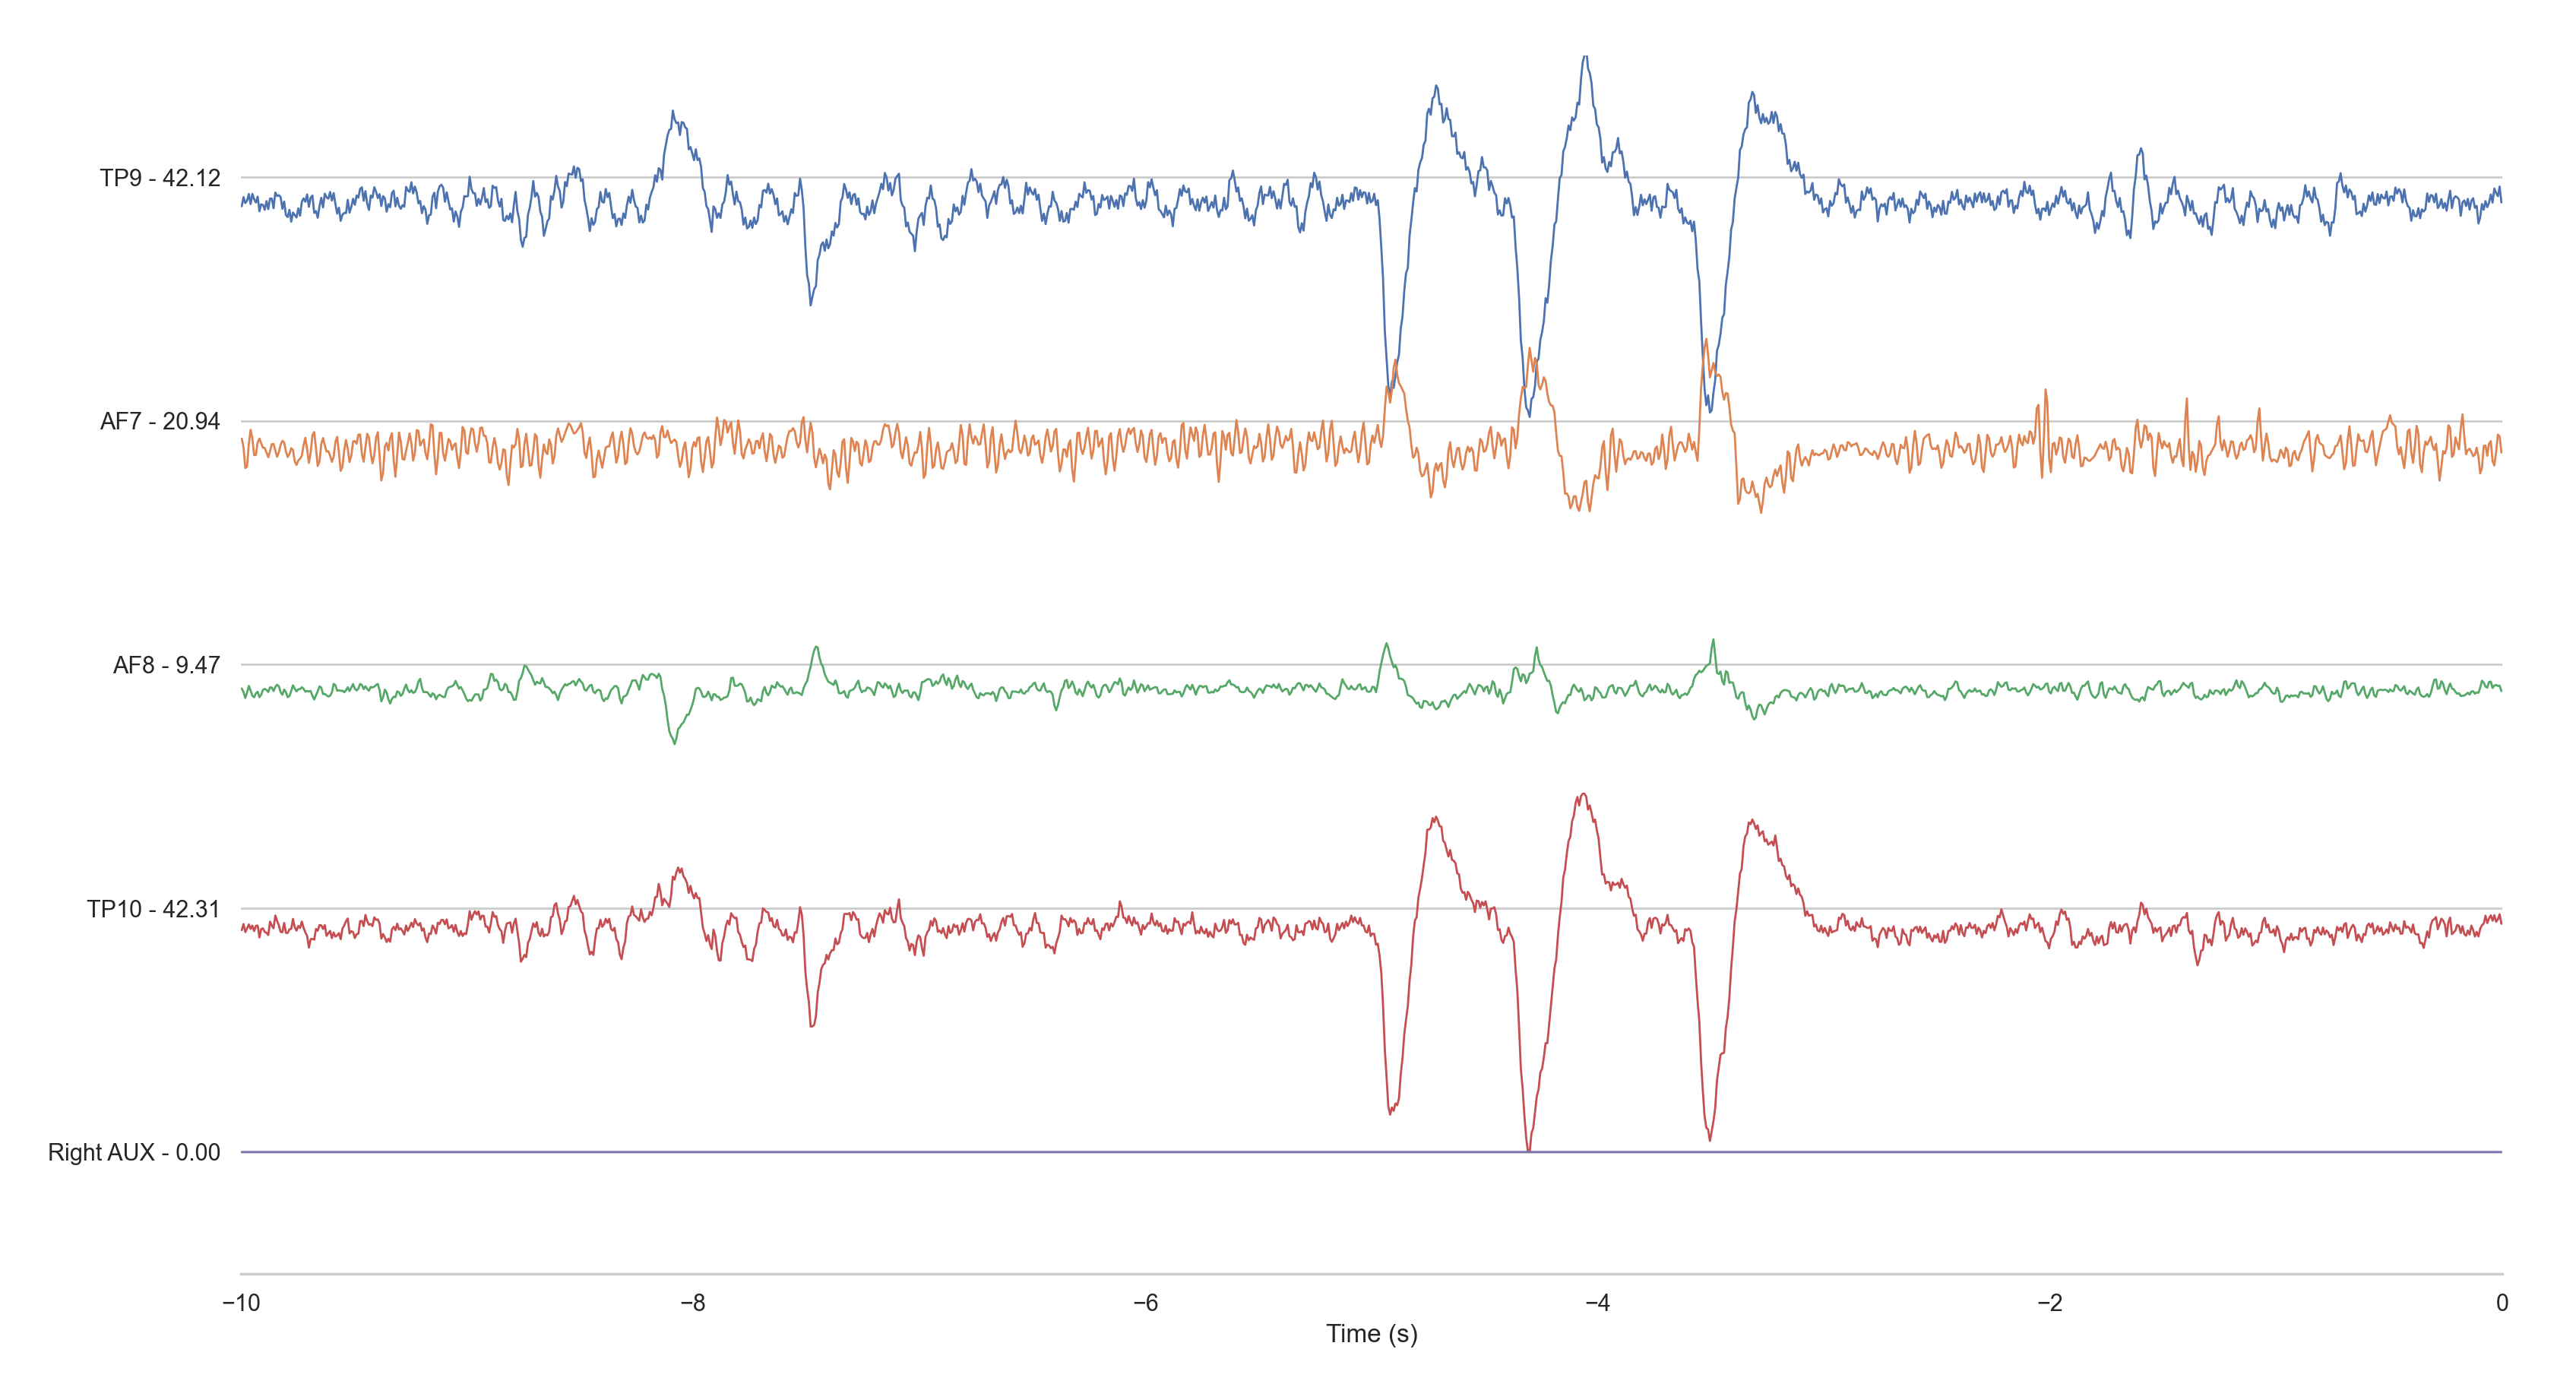
\includegraphics[trim=60 50 50 60,clip,width=22cm]{img/muselsl-signal.png}
            \end{center}
            \caption{EEG signal viewed with muse-lsl. There are 3 eye blinks identifiable around $\SI{-4}{\second}$.\\ The signal has been bandpass filtered to eliminate noise.}\label{fig:muselsl-signal}
        \end{figure}
    \end{landscape}

\section{Machine Learning}

    Machine learning on EEG data utilizes several domain-specific methods, often similar to other methods for time-series data in general. However, some methods differ by taking advantage of the spatial information that is available through the analysis of interdependence between multiple EEG channels~\cite{lotte_review_2018}.

    Methods used in analysis and classification of EEG data include Linear Discriminant Analysis (LDA), Common Spatial Pattern (CSP) filters~\cite{barachant_common_2010}, spectral density estimation (bandpower features), and the computation of covariance matrices to estimate interdependencies between channels. The underlying ML algorithms being trained on the features are often off-the-shelf logistic regression, support vector machines, random forests, etc. Some domain adaptations are found in more complex models like neural networks.

    Furthermore, preprocessing methods include bandpass filtering, windowing, and various tricks for channel selection (in high-density setups). With the use of these methods, we can preprocess the data, compute features, and train our classifiers.

    In our study, we will primarily be using Riemannian methods, and compare them to a common bandpower-features approach (used by Fucci et al.) as our baseline.

    %For logistic regression, the \emph{log loss} function $L$ is defined as:

    %\[ L(x, y') = \sum_{(x,y) \in D} -y \log y' - (1 - y) \log(1 - y')\]

    \subsection{Riemannian geometry}\label{section:riemannian-theory}

        %\add[inline]{Explanation of Riemannian geometry, from \href{https://colab.research.google.com/drive/1y9tq7-lJwusxtVgpB38y-p1pYw7hg0iu}{this tutorial we're working on}}

        EEG decoding approaches based on Riemannian geometry have led to state-of-the-art classification performance on many tasks~\cite{lotte_review_2018}. The idea behind it is to take advantage of the spatial structure of EEG, i.e.\ the fact that there are multiple channels which co-vary in specific ways.

        The Riemannian distance metric $\delta_G$ for two symmetric positive definite matrices $\mathrm{A}$ and $\mathrm{B}$ (such as covariance matrices) is~\cite{grafarend_metric_2003}:

        \[ \delta_G(\mathrm{A}, \mathrm{B}) = \sqrt{\sum_{i=1}^N \ln^2 \lambda_i (\mathrm{A}, \mathrm{B}) } \]

        Where $ \mathrm{\lambda}_i(\mathrm{A}, \mathrm{B}) $ are the eigenvalues from $|\mathrm{\lambda}\mathrm{A} - \mathrm{B}| = 0$.

        The naive Riemannian approach using \emph{Minimum Distance to Mean} (MDM) starts with computing the covariance matrix for each trial, and then estimating a mean covariance matrix for each class (the class centroid) using the Riemannian distance metric $\delta_G$. When classification is performed, the distance between the new covariance matrix and the class centroids is estimated using the Riemannian distance metric, and the new covariance matrix is classified according to which class centroid is closest.

        To allow for use of other classification approaches in the final step, such as logistic regression and SVMs, we can project our covariance matrices onto a tangent space (a schematic representation of this can be seen in Figure~\ref{figure:tangent-space}). Once projected onto this tangent space, our covariance matrices can be compared fairly well using the standard Euclidean distance metric, letting us use common methods which do not employ the Riemannian distance metric~\cite{congedo_riemannian_2017}.

        \begin{figure}[h]
    \centering
    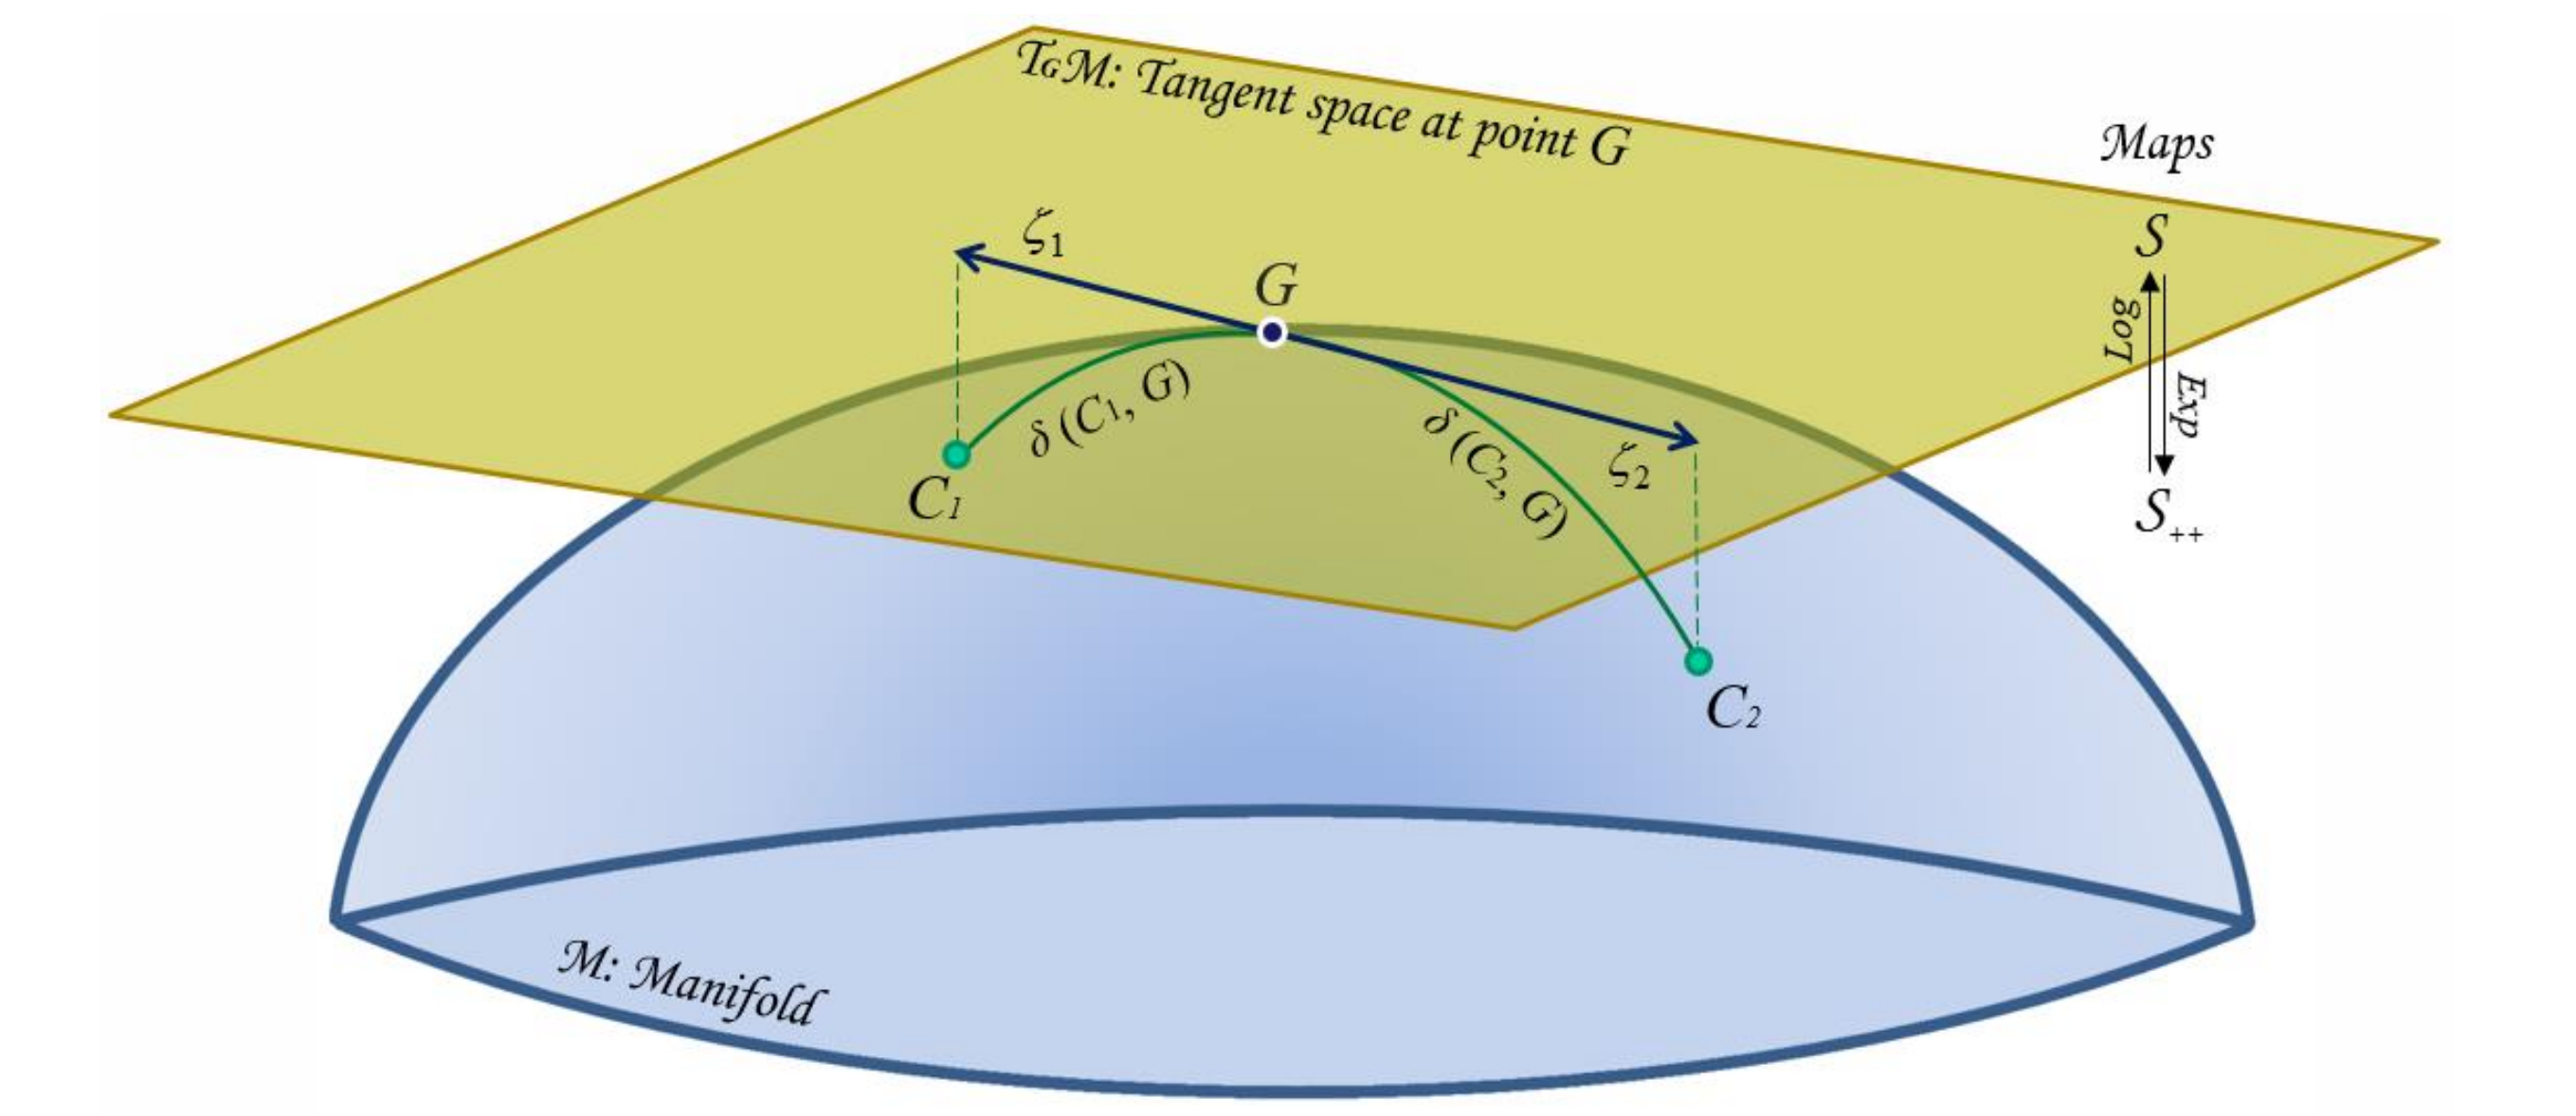
\includegraphics[width=0.6\textwidth]{img/riemannian-tangent-space.png}
    \caption{Schematic representation of the symmetric positive definite matrix manifold, the geometric mean $G$ of two points and the tangent space at $G$. The geometric mean of these points is the midpoint on the geodesic connecting $C_1$ and $C_2$, i.e.\ it minimizes the sum of the two squared distances. The map from the tangent space to the manifold is an exponential map. The inverse map is a logarithmic map.}\label{figure:tangent-space}
    \source{Congedo et al.~\cite{congedo_riemannian_2017}}
\end{figure}


    \begin{comment}
    \subsection{Neural networks}
        Many state-of-the-art models in the field of EEG are deep-learning based models, usually employing convolutional neural networks (CNNs).
    \end{comment}
